\documentclass{article}
\usepackage[utf8]{inputenc}
\usepackage{amsmath}
\usepackage{amssymb}
\usepackage{graphicx}
\usepackage{tabularx}
\usepackage{booktabs}
\usepackage[english]{babel}
\usepackage{setspace}
\usepackage{geometry}
\usepackage{float}
\usepackage{url}
\usepackage{listings}
\usepackage{xcolor}
\usepackage{longtable}
\usepackage{tikz}
\usetikzlibrary{positioning, calc}
\usepackage[justification=centering]{caption}

\lstset{
    basicstyle=\ttfamily\small,
    backgroundcolor=\color{gray!10},
    frame=single,
    breaklines=true,
    columns=fullflexible
}

% APA style formatting
\geometry{a4paper, margin=1in}
\setstretch{1.5}
\setlength{\emergencystretch}{3em} % lets long \texttt names wrap without overflowing the margin
\captionsetup[table]{labelfont=bf, justification=centering, singlelinecheck=false}
\captionsetup[longtable]{labelfont=bf, justification=centering, singlelinecheck=false}
\captionsetup[figure]{font=small, labelfont=bf, justification=centering, singlelinecheck=false}

% Notation helpers
\newcommand{\R}{\mathbb{R}}
\newcommand{\slog}{\operatorname{slog}}
\newcommand{\clip}{\operatorname{clip}}
\newcommand{\ind}{\mathbf{1}}

\title{Machine Learning for Customer Churn Prediction}
\author{Nelson David Posso Suarez \\ Javier Alejandro Penagos Hernandez \\ Nicolas Castro Rivera }
\date{}

\begin{document}

\maketitle

% ─────────────────────────────────────────────
\section{Data Preparation}
% ─────────────────────────────────────────────

In this workshop the churn problem is approached from a different angle. Instead of summarising each subscriber into a single tabular row, as in Workshop~1, we use the dates in the dataset to treat churn prediction as a \textbf{sequence problem}: each subscriber is represented by the day-by-day evolution of their listening activity and subscription status. This requires transforming the raw data in a different way from the previous workshop. The pipeline is implemented in \path{workshops/w2/w2_sequence_preprocessing.ipynb} and the modules under \path{workshops/w2/src/data_processing/}.

% ─────────────────────────────────────────────
\subsection{Structure of the Raw Data}
% ─────────────────────────────────────────────

The dataset covers approximately 2015 to 2017 and contains the history of each subscriber's transactions and music listening logs. Three of the raw tables are used to build the sequences: the labelled cohorts (Table~\ref{tab:w2_schema_train}), the daily listening logs (Table~\ref{tab:w2_schema_logs}) and the payment transactions (Table~\ref{tab:w2_schema_transactions}). The member demographics table is not used in this workshop.

\begin{table}[H]
\centering
\renewcommand{\arraystretch}{1.3}
\begin{tabularx}{\textwidth}{|l|X|l|}
\hline
\textbf{Feature} & \textbf{Description} & \textbf{Data type} \\ \hline
msno      & Hashed subscriber identifier (primary key) & \texttt{str} \\ \hline
is\_churn & Churn label: 1 if the user did not renew within 30 days of expiry, 0 otherwise & \texttt{int8} \\ \hline
\end{tabularx}
\caption{Schema of \texttt{train.csv} (February cohort) and \texttt{train\_v2.csv} (March cohort).}
\label{tab:w2_schema_train}
\end{table}

\begin{table}[H]
\centering
\renewcommand{\arraystretch}{1.3}
\begin{tabularx}{\textwidth}{|l|X|l|}
\hline
\textbf{Feature} & \textbf{Description} & \textbf{Data type} \\ \hline
msno        & Hashed subscriber identifier (foreign key) & \texttt{str} \\ \hline
date        & Listening date in YYYYMMDD format & \texttt{int32} \\ \hline
num\_25     & Number of songs played less than 25\% of their duration & \texttt{int32} \\ \hline
num\_50     & Number of songs played between 25\% and 50\% of their duration & \texttt{int32} \\ \hline
num\_75     & Number of songs played between 50\% and 75\% of their duration & \texttt{int32} \\ \hline
num\_985    & Number of songs played between 75\% and 98.5\% of their duration & \texttt{int32} \\ \hline
num\_100    & Number of songs played at least 98.5\% of their duration & \texttt{int32} \\ \hline
num\_unq    & Number of unique songs played on that day & \texttt{int32} \\ \hline
total\_secs & Total seconds of music listened to on that day & \texttt{float64} \\ \hline
\end{tabularx}
\caption{Schema of \texttt{user\_logs.csv} and \texttt{user\_logs\_v2.csv}.}
\label{tab:w2_schema_logs}
\end{table}

\begin{table}[H]
\centering
\renewcommand{\arraystretch}{1.3}
\begin{tabularx}{\textwidth}{|l|X|l|}
\hline
\textbf{Feature} & \textbf{Description} & \textbf{Data type} \\ \hline
msno                     & Hashed subscriber identifier (foreign key) & \texttt{str} \\ \hline
payment\_method\_id      & Payment method encoded as an integer code & \texttt{int8} \\ \hline
payment\_plan\_days      & Number of days in the purchased subscription plan & \texttt{int16} \\ \hline
plan\_list\_price        & Listed price of the plan in New Taiwan Dollars (NTD) & \texttt{int16} \\ \hline
actual\_amount\_paid     & Amount actually paid by the subscriber in NTD & \texttt{int16} \\ \hline
is\_auto\_renew          & Automatic renewal flag (1 = yes, 0 = no) & \texttt{int8} \\ \hline
transaction\_date        & Date of the transaction in YYYYMMDD format & \texttt{int32} \\ \hline
membership\_expire\_date & Membership expiration date after the transaction in YYYYMMDD format & \texttt{int32} \\ \hline
is\_cancel               & Cancellation flag (1 = yes, 0 = no) & \texttt{int8} \\ \hline
\end{tabularx}
\caption{Schema of \texttt{transactions.csv} and \texttt{transactions\_v2.csv}.}
\label{tab:w2_schema_transactions}
\end{table}

% ─────────────────────────────────────────────
\subsection{Tensor Construction}
% ─────────────────────────────────────────────

\subsubsection{Temporal Split and Window Overlap}

Each cohort $c$ is defined by a cutoff date $\tau_c$, the last day whose information may be used. Its sequence window contains the $L = 90$ consecutive calendar days that end on the cutoff:
\begin{equation}
W_c = \{\, \tau_c - 89,\; \tau_c - 88,\; \dots,\; \tau_c \,\}, \qquad |W_c| = L = 90 .
\end{equation}
A calendar date $d \in W_c$ is mapped to the day index
\begin{equation}
t(d) = d - (\tau_c - 89) \in \{0, 1, \dots, 89\},
\end{equation}
so $t = 0$ is the oldest day of the window and $t = 89$ is the cutoff. Table~\ref{tab:w2_cohorts} lists the two cohorts.

\begin{table}[H]
\centering
\renewcommand{\arraystretch}{1.3}
\begin{tabular}{|l|l|l|l|r|r|}
\hline
\textbf{Cohort} & \textbf{Role} & \textbf{Window $W_c$} & \textbf{Target} & \textbf{Users $N_c$} & \textbf{Churn rate} \\ \hline
\texttt{train\_feb} & Training & 2016-11-03 to 2017-01-31 & February 2017 & 992{,}931 & 6.4\% \\ \hline
\texttt{test}       & Test     & 2016-12-01 to 2017-02-28 & March 2017    & 970{,}960 & 9.0\% \\ \hline
\end{tabular}
\caption{Labelled cohorts, their 90-day windows and churn targets.}
\label{tab:w2_cohorts}
\end{table}

We build the training tensor from each user's activity between 2016-11-03 and 2017-01-31, with February 2017 churn as the target. The test tensor uses the window from 2016-12-01 to 2017-02-28, with March 2017 churn as the target. The two windows overlap by 62 days (2016-12-01 to 2017-01-31), as shown in Figure~\ref{fig:w2_overlap}.

\begin{figure}[H]
\centering
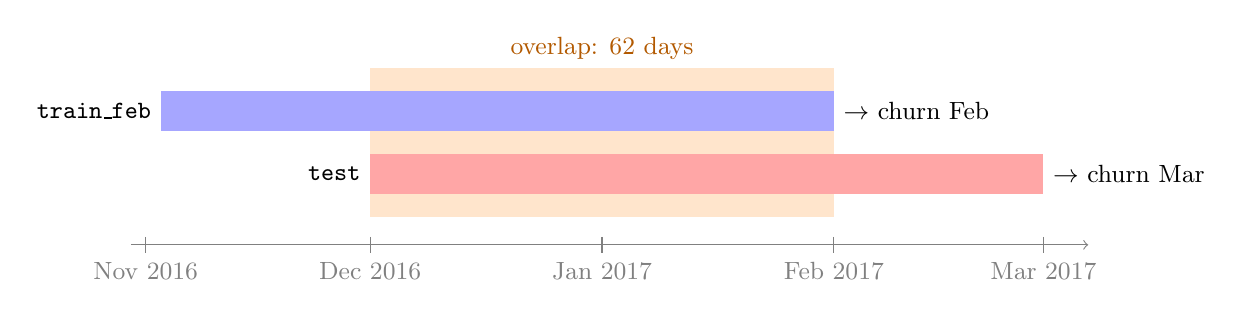
\begin{tikzpicture}[x=0.095cm, y=1cm, font=\small]
    % Day 0 = 2016-11-03. Month starts: Nov 1 = -2, Dec 1 = 28, Jan 1 = 59, Feb 1 = 90, Mar 1 = 118
    \draw[->, gray] (-4,0) -- (124,0);
    \foreach \x/\lbl in {-2/Nov 2016, 28/Dec 2016, 59/Jan 2017, 90/Feb 2017, 118/Mar 2017} {
        \draw[gray] (\x,0.1) -- (\x,-0.1);
        \node[below, gray] at (\x,-0.1) {\lbl};
    }
    % Overlap band
    \fill[orange!20] (28,0.35) rectangle (90,2.25);
    \node[orange!70!black] at (59,2.5) {overlap: 62 days};
    % Train window
    \fill[blue!35] (0,1.45) rectangle (90,1.95);
    \node[left] at (0,1.7) {\texttt{train\_feb}};
    \node[right] at (90,1.7) {$\rightarrow$ churn Feb};
    % Test window
    \fill[red!35] (28,0.65) rectangle (118,1.15);
    \node[left] at (28,0.9) {\texttt{test}};
    \node[right] at (118,0.9) {$\rightarrow$ churn Mar};
\end{tikzpicture}
\caption{90-day windows of the two cohorts. Each window ends at its cutoff (2017-01-31 and 2017-02-28) and is followed by its target month.}
\label{fig:w2_overlap}
\end{figure}

This overlap is intentional. It follows from using a fixed-length lookback window that advances one month at a time, which is how a subscription service would score its customers in production. Each month, the model receives the most recent 90 days of behaviour and predicts whether the customer will renew in the following month, so consecutive scoring windows necessarily share most of their history.

The overlap does not leak target information. Every feature is computed using only data up to its window's cutoff, and the labels belong to different, non-overlapping periods (February for training, March for testing). During training the model never observes the March outcome, nor any activity after 2017-01-31. The test set therefore measures forward-looking temporal generalisation: how well a model trained on one month's snapshot predicts the next month's churn, including any behavioural drift between the two months.

Many users appear in both cohorts (881{,}701 of the February users are also in the March cohort), as they would in real monthly scoring. A shared integer identifier \texttt{uid} is assigned over the union of both cohorts (1{,}082{,}190 unique users) and is used only to join each user with their logs and transactions. Each cohort keeps its own complete list of users, its own row order and its own labels: a user present in only one cohort appears only in that cohort's tensor, and a user present in both appears twice, with a different cutoff, sequence and label each time. Our results should therefore be read as performance on an existing customer base rather than on entirely unseen users.

\subsubsection{Cleaning}

\paragraph{Transactions.} Both transaction files are concatenated, restricted to the target users and to transactions on or before the cutoff. Exact duplicates are then removed: two rows are considered duplicates when the user (\texttt{msno}) and all eight transaction fields (\texttt{payment\_method\_id}, \texttt{payment\_plan\_days}, \texttt{plan\_list\_price}, \texttt{actual\_amount\_paid}, \texttt{is\_auto\_renew}, \texttt{transaction\_date}, \texttt{membership\_expire\_date}, \texttt{is\_cancel}) are equal. Only the first copy is kept. Two rows on the same day with different values are treated as different payments and both are kept.

\paragraph{Listening logs.} The raw logs may contain several rows for the same user and day. Before aggregation, negative counters are clipped to zero and non-finite values of \texttt{total\_secs} are replaced by zero. The rows of the same user and day are then summed into a single row. For example, if user $A$ has three rows on 2017-02-01, with \texttt{num\_25} equal to 3, 2 and 1, the aggregated row has \texttt{num\_25} $= 6$; the other counters are summed in the same way. Formally, for user $i$, day $d$ and counter $k$:
\begin{equation}
v_{i,d,k} = \sum_{r \in R_{i,d}} \max(0,\, v_{r,k}),
\end{equation}
where $R_{i,d}$ is the set of raw log rows of user $i$ on day $d$. The number of raw rows $|R_{i,d}|$ is kept to define the activity flag.

\subsubsection{Listening Channels}

The aggregated logs are placed into the window. Days without any log row are filled with zeros. The seven counters are transformed with $\log(1+x)$ to compress their heavy-tailed distribution; standard scaling is fitted later, on the training split only, inside the model notebook. An eighth channel, \texttt{active}, indicates whether a log row exists for that day, independently of the counter values:
\begin{equation}
x_{i,t,k} = \log\!\left(1 + v_{i,d,k}\right), \quad k = 1,\dots,7, \qquad
a_{i,t} = \ind\!\left[\,|R_{i,d}| > 0\,\right],
\end{equation}
with $t = t(d)$. A day with a log row where every counter is zero is still active, which distinguishes ``logged in but did not listen'' from ``no record''. Table~\ref{tab:w2_listening} lists the listening channels.

\begin{table}[H]
\centering
\renewcommand{\arraystretch}{1.3}
\begin{tabularx}{\textwidth}{|c|l|X|l|}
\hline
\textbf{Index} & \textbf{Channel} & \textbf{Description} & \textbf{Encoding} \\ \hline
0 & num\_25     & Songs played less than 25\% & $\log(1+x)$ \\ \hline
1 & num\_50     & Songs played 25--50\%       & $\log(1+x)$ \\ \hline
2 & num\_75     & Songs played 50--75\%       & $\log(1+x)$ \\ \hline
3 & num\_985    & Songs played 75--98.5\%     & $\log(1+x)$ \\ \hline
4 & num\_100    & Songs played at least 98.5\% & $\log(1+x)$ \\ \hline
5 & num\_unq    & Unique songs played         & $\log(1+x)$ \\ \hline
6 & total\_secs & Seconds listened            & $\log(1+x)$ \\ \hline
7 & active      & 1 if a log row exists for the day, 0 otherwise & flag \\ \hline
\end{tabularx}
\caption{Listening channels (8) of the sequence tensor.}
\label{tab:w2_listening}
\end{table}

\subsubsection{Transaction Channels: Events and States}

The tensor is completed with twelve transaction channels, divided into two groups:

\begin{itemize}
    \item \textbf{Events} encode what happened on a specific day. They are written only on the days with at least one payment and are zero on every other day.
    \item \textbf{States} encode the subscription status known at the end of a specific day. They are carried forward to the following days until the next payment updates them.
\end{itemize}

First, the transactions of each user are aggregated per day. Event values are summed over all payments of the day. State values (cancellation, auto-renewal and expiry date) are taken from the last record of that day in source order, and a flag marks the day as ambiguous when the records of the same day disagree on any of these three values.

\paragraph{Payments before the window.} Only the \textbf{latest payment day before the window} is kept from the earlier history; all earlier payments are summarised by that single record. This record initialises the state at $t = 0$ but does not create an event inside the window. A payment on day $t$ writes the event channels on day $t$ and updates the state from day $t$ onward. Future payments never modify earlier days, which guarantees that the tensor is causal. This property is verified in the notebook by comparing the vectorised builder against a day-by-day reference implementation and checking that adding a later payment leaves every earlier day unchanged.

Formally, let $P_i$ be the set of payment days of user $i$ up to the cutoff, and let
\begin{equation}
s_i(t) = \max \{\, p \in P_i : p \le d_t \,\}
\end{equation}
be the most recent payment day known on day $d_t$ (possibly before the window). The state is known when $s_i(t)$ exists, and the recency and expiry channels are
\begin{align}
\text{tx\_days\_since\_last}_{i,t} &= \log\!\Big(1 + \clip\big(d_t - s_i(t),\, 0,\, 3650\big)\Big), \\
\text{tx\_days\_to\_expire}_{i,t}  &= \slog\!\Big(\clip\big(e_i(t) - d_t,\, -3650,\, 3650\big)\Big),
\end{align}
where $e_i(t)$ is the membership expiry date recorded on day $s_i(t)$, and $\slog(x) = \operatorname{sign}(x)\log(1 + |x|)$ is the signed logarithm, used for quantities that can be negative (an already expired membership, or a negative amount paid). When the state is not yet known, all state channels are zero.

\paragraph{Worked example.} Consider a user of the \texttt{test} cohort, whose window starts on 2016-12-01 ($t = 0$). The user paid on 2016-11-20, before the window, with auto-renewal disabled and a membership that expires on 2016-12-20, and made no further payments. The pre-window payment initialises the state, so $s_i(t) = \text{2016-11-20}$ and $e_i(t) = \text{2016-12-20}$ for every day of the window, and no event is written on any day. Table~\ref{tab:w2_example} shows the two channels on three days. On day 19 the membership expires and \texttt{tx\_days\_to\_expire} is zero; from day 20 on it is negative, a strong signal that the user has not renewed. These values were obtained by running this user through the same builder used for the export.

\begin{table}[H]
\centering
\renewcommand{\arraystretch}{1.3}
\begin{tabular}{|c|c|c|c|c|c|}
\hline
\textbf{Day $t$} & \textbf{Date $d_t$} & $d_t - s_i(t)$ & \textbf{tx\_days\_since\_last} & $e_i(t) - d_t$ & \textbf{tx\_days\_to\_expire} \\ \hline
0  & 2016-12-01 & 11 & $\log(1 + 11) = 2.48$ & 19  & $\slog(19) = 3.00$ \\ \hline
19 & 2016-12-20 & 30 & $\log(1 + 30) = 3.43$ & 0   & $\slog(0) = 0.00$ \\ \hline
24 & 2016-12-25 & 35 & $\log(1 + 35) = 3.58$ & $-5$ & $\slog(-5) = -1.79$ \\ \hline
\end{tabular}
\caption{Recency and expiry channels for a user whose only payment (2016-11-20, expiring 2016-12-20) falls before the \texttt{test} window.}
\label{tab:w2_example}
\end{table}

Table~\ref{tab:w2_transactions} describes each transaction channel.

\renewcommand{\arraystretch}{1.3}
\begin{longtable}{|c|l|c|p{6.2cm}|l|}
\hline
\textbf{Index} & \textbf{Channel} & \textbf{Group} & \textbf{Description} & \textbf{Encoding} \\ \hline
\endfirsthead
\hline
\textbf{Index} & \textbf{Channel} & \textbf{Group} & \textbf{Description} & \textbf{Encoding} \\ \hline
\endhead
\hline
\multicolumn{5}{r}{\small\textit{Continued on next page}} \\
\endfoot
\hline
\caption{Transaction channels (12) of the sequence tensor.}
\label{tab:w2_transactions}
\endlastfoot
8  & tx\_count               & Event & Number of payments on the day & $\log(1+x)$ \\ \hline
9  & tx\_paid\_sum           & Event & Total amount paid on the day (NTD) & $\slog(x)$ \\ \hline
10 & tx\_plan\_days\_sum     & Event & Total plan days purchased on the day & $\log(1+x)$ \\ \hline
11 & tx\_cancel\_count       & Event & Number of cancellation records on the day & $\log(1+x)$ \\ \hline
12 & tx\_auto\_renew\_count  & Event & Number of auto-renew records on the day & $\log(1+x)$ \\ \hline
13 & tx\_state\_known        & State & 1 once at least one payment has been observed up to the day, including the pre-window payment & flag \\ \hline
14 & tx\_last\_is\_cancel    & State & Cancellation flag of the most recent payment day & flag \\ \hline
15 & tx\_last\_is\_auto\_renew & State & Auto-renew flag of the most recent payment day & flag \\ \hline
16 & tx\_days\_since\_last   & State & Days since the most recent payment, clipped to $[0, 3650]$ & $\log(1+x)$ \\ \hline
17 & tx\_days\_to\_expire    & State & Membership expiry minus the current day, clipped to $[-3650, 3650]$ & $\slog(x)$ \\ \hline
18 & tx\_expiry\_known       & State & 1 if the expiry date of the most recent payment is valid & flag \\ \hline
19 & tx\_state\_ambiguous    & State & 1 if the records of the most recent payment day disagree on cancellation, auto-renewal or expiry & flag \\ \hline
\end{longtable}

\subsubsection{Resulting Tensor}

For each user $i$ of cohort $c$, the 20 channels are stacked into a matrix whose rows are the 90 days, ordered from oldest to newest, and whose columns are the channels in the order of Tables~\ref{tab:w2_listening} and~\ref{tab:w2_transactions}:
\begin{equation}
X_i^{(c)} =
\begin{bmatrix}
x_{i,0,0}  & x_{i,0,1}  & \cdots & x_{i,0,19} \\
x_{i,1,0}  & x_{i,1,1}  & \cdots & x_{i,1,19} \\
\vdots     & \vdots     & \ddots & \vdots \\
x_{i,89,0} & x_{i,89,1} & \cdots & x_{i,89,19}
\end{bmatrix}
\in \R^{L \times F}, \qquad L = 90,\; F = 20 .
\end{equation}
Stacking the $N_c$ users of the cohort gives the cohort tensor
\begin{equation}
\mathcal{X}^{(c)} = \big[\, X_1^{(c)}, X_2^{(c)}, \dots, X_{N_c}^{(c)} \,\big] \in \R^{N_c \times L \times F},
\end{equation}
together with the label vector $y^{(c)} \in \{0,1\}^{N_c}$, aligned so that position $i$ of $y^{(c)}$ is the label of $X_i^{(c)}$. The channel dimension splits into three blocks:
\begin{equation}
X_i^{(c)} = \big[\; \underbrace{X_i^{\text{listen}}}_{\R^{90 \times 8}} \;\big|\; \underbrace{X_i^{\text{event}}}_{\R^{90 \times 5}} \;\big|\; \underbrace{X_i^{\text{state}}}_{\R^{90 \times 7}} \;\big].
\end{equation}

In this way we obtain $\mathcal{X}^{(\text{train\_feb})} \in \R^{992{,}931 \times 90 \times 20}$ and $\mathcal{X}^{(\text{test})} \in \R^{970{,}960 \times 90 \times 20}$. The tensors are stored as \texttt{float16} arrays (\texttt{seq\_lstm\_train\_feb.npy} and \texttt{seq\_lstm\_test.npy}, about 3.5~GB each) with their labels in \texttt{labels\_<cohort>.parquet}, in the directory \texttt{workshops/w2/export-sequential-v5/}. Before export, an audit rejects the tensor if any of the following fails: the expected shape, finite values, binary flags, non-negative counts and recency, zero event channels on days without a payment, and zero state channels before the state is known.

% ─────────────────────────────────────────────
\section{Model}
% ─────────────────────────────────────────────

We use a recurrent neural network, the Long Short-Term Memory network (LSTM). We choose this architecture because it is designed for ordered sequences: it reads the 90 days one at a time and keeps an internal memory of the customer's past behaviour, which suits the daily tensors built in the previous section. The model is implemented in PyTorch in the class \texttt{LSTMModel} (\path{workshops/w2/src/models/lstm/model.py}). Defining it as a class lets us reuse the same model and change its size (number of layers and hidden units) without modifying the code. The training and evaluation are orchestrated in \path{workshops/w2/w2_neural_models.ipynb}.

\subsection{Architecture}

The architecture has the following layers (Figure~\ref{fig:w2_arch}):

\begin{itemize}
    \item \textbf{Input layer.} A batch of users taken from the tensor built before, with shape $(B, 90, 20)$: $B$ users, 90 days and 20 channels. Each day $t$ of user $i$ is the vector $x_{i,t} \in \R^{20}$.
    \item \textbf{Hidden dimension} (\texttt{hidden\_dim}). The number of units in the hidden state $h_t \in \R^{H}$ of each LSTM layer. It sets how much information the network can store about the customer.
    \item \textbf{Layer dimension} (\texttt{layer\_dim}). The number of stacked LSTM layers, between 2 and 4. The first layer reads the 20 channels of each day; each following layer reads the hidden states of the layer below. Inside each cell, the gates use the sigmoid function and the candidate memory and output use $\tanh$, which introduces the nonlinearity and keeps the hidden state bounded in $[-1, 1]$.
    \item \textbf{Batch normalisation layer.} After the 90 days, the output of the last layer on the last day, $h_{90} \in \R^{H}$, has shape $(B, H)$. This vector summarises the customer's behaviour over the 90 days. \texttt{BatchNorm1d} normalises it across the batch, which stabilises the training.
    \item \textbf{Output layer.} A linear layer applies the transformation $z = w^\top \tilde{h}_{90} + b$ and produces one value per user, the \emph{logit} $z \in \R$.
\end{itemize}

For each day, an LSTM layer updates its memory cell $c_t$ and hidden state $h_t$ with
\begin{align}
f_t &= \sigma(W_f x_t + U_f h_{t-1} + b_f), &
i_t &= \sigma(W_i x_t + U_i h_{t-1} + b_i), &
o_t &= \sigma(W_o x_t + U_o h_{t-1} + b_o), \\
\tilde{c}_t &= \tanh(W_c x_t + U_c h_{t-1} + b_c), &
c_t &= f_t \odot c_{t-1} + i_t \odot \tilde{c}_t, &
h_t &= o_t \odot \tanh(c_t),
\end{align}
where $f_t$, $i_t$ and $o_t$ are the forget, input and output gates, $\sigma$ is the sigmoid function and $\odot$ is the element-wise product. The states start at $h_0 = c_0 = 0$. The model output and the churn probability are
\begin{equation}
z_i = w^\top \operatorname{BN}\big(h_{i,90}\big) + b, \qquad \hat{p}_i = \sigma(z_i) = \frac{1}{1 + e^{-z_i}} .
\end{equation}

\begin{figure}[H]
\centering
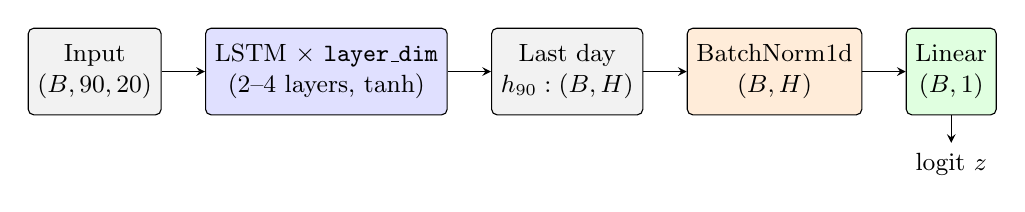
\begin{tikzpicture}[
    box/.style={draw, rounded corners=2pt, minimum height=1.1cm, align=center, font=\small, fill=#1},
    box/.default={gray!10},
    >=stealth, node distance=0.55cm
]
    \node[box] (in) {Input\\$(B, 90, 20)$};
    \node[box=blue!12, right=of in] (lstm) {LSTM $\times$ \texttt{layer\_dim}\\(2--4 layers, $\tanh$)};
    \node[box, right=of lstm] (last) {Last day\\$h_{90}: (B, H)$};
    \node[box=orange!15, right=of last] (bn) {BatchNorm1d\\$(B, H)$};
    \node[box=green!12, right=of bn] (fc) {Linear\\$(B, 1)$};
    \draw[->] (in) -- (lstm);
    \draw[->] (lstm) -- (last);
    \draw[->] (last) -- (bn);
    \draw[->] (bn) -- (fc);
    \node[below=0.35cm of fc, font=\small] (out) {logit $z$};
    \draw[->] (fc) -- (out);
\end{tikzpicture}
\caption{LSTM architecture. $B$ is the batch size and $H$ the hidden dimension. The sigmoid is applied to the logit inside the loss during training and explicitly at prediction time.}
\label{fig:w2_arch}
\end{figure}

\subsection{Loss Function and Optimiser}

Since churn is a binary classification problem, we use the binary cross-entropy loss. In PyTorch it is defined as \texttt{criterion = nn.BCEWithLogitsLoss()}. This function receives the logit $z_i$ and applies the sigmoid internally, so the model does not include a sigmoid layer. Combining both operations in one function is numerically stable: it never evaluates $\log(0)$ when the sigmoid saturates. For a batch of $B$ users the loss is
\begin{equation}
\mathcal{L} = -\frac{1}{B} \sum_{i=1}^{B} \Big[ y_i \log \sigma(z_i) + (1 - y_i) \log\big(1 - \sigma(z_i)\big) \Big].
\end{equation}
At prediction time, where there is no loss, the probability is obtained explicitly with \path{torch.sigmoid(logits)}.

\paragraph{Backpropagation.} Figure~\ref{fig:w2_backprop} summarises how the network learns. In the \textbf{forward pass} (black), each layer transforms the output of the previous one:
\begin{itemize}
    \item \textbf{Input:} the 90 days of the user, each a vector of 20 channels.
    \item \textbf{LSTM:} reads the days in order and updates its hidden state, which accumulates the customer's history up to day 90.
    \item \textbf{BatchNorm:} normalises the final hidden state $h_{90}$ so that its scale stays stable during training.
    \item \textbf{Linear:} combines the normalised hidden state into a single score, the logit $z$.
    \item \textbf{Sigmoid:} turns the logit into a churn probability $\hat p$ between 0 and 1.
    \item \textbf{BCE loss:} compares $\hat p$ with the true label $y$ and measures the error.
\end{itemize}
In the \textbf{backward pass} (red), the error travels in the opposite direction, from the loss to the input. Each layer receives how much it contributed to the error and passes it on to the layer before. Inside the LSTM, the error also travels back through the 90 days, from the last day to the first. With this information, AdamW adjusts the weights of every layer to reduce the error in the next batch.

\begin{figure}[H]
\centering
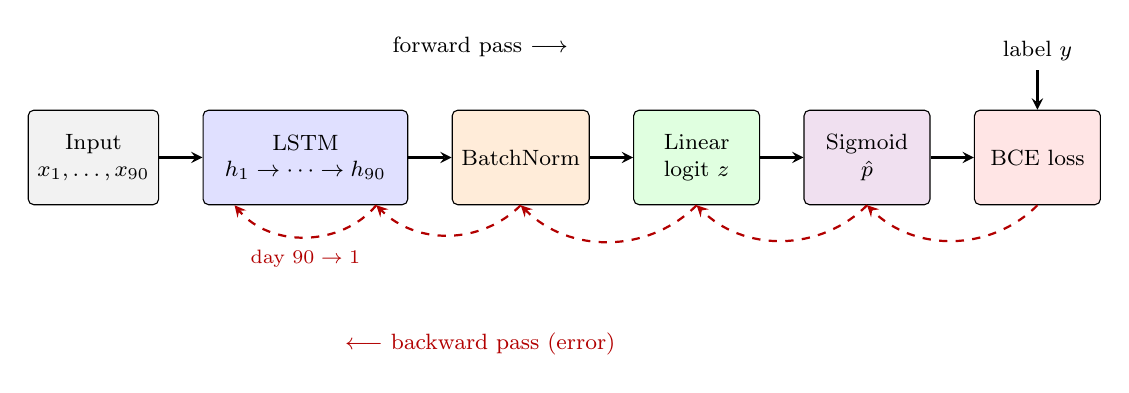
\begin{tikzpicture}[
    op/.style={draw, rounded corners=2pt, minimum height=1.2cm, minimum width=1.6cm, align=center, font=\footnotesize, fill=#1},
    op/.default={gray!10},
    fwd/.style={->, >=stealth, thick},
    bwd/.style={->, >=stealth, thick, red!70!black, dashed},
    node distance=0.55cm
]
    % Forward pass
    \node[op] (x) {Input\\$x_1, \dots, x_{90}$};
    \node[op=blue!12, right=of x, minimum width=2.6cm] (lstm) {LSTM\\$h_1 \to \cdots \to h_{90}$};
    \node[op=orange!15, right=of lstm] (bn) {BatchNorm};
    \node[op=green!12, right=of bn] (fc) {Linear\\logit $z$};
    \node[op=violet!12, right=of fc] (sig) {Sigmoid\\$\hat p$};
    \node[op=red!10, right=of sig] (loss) {BCE loss};
    \node[above=0.5cm of loss, font=\footnotesize] (y) {label $y$};

    \draw[fwd] (x) -- (lstm);
    \draw[fwd] (lstm) -- (bn);
    \draw[fwd] (bn) -- (fc);
    \draw[fwd] (fc) -- (sig);
    \draw[fwd] (sig) -- (loss);
    \draw[fwd] (y) -- (loss);
    \node[font=\footnotesize, anchor=south] at ($(x.north)!0.5!(sig.north) + (0,0.55)$) {forward pass $\longrightarrow$};

    % Backward pass
    \draw[bwd] (loss.south) to[bend left=45] (sig.south);
    \draw[bwd] (sig.south) to[bend left=45] (fc.south);
    \draw[bwd] (fc.south) to[bend left=45] (bn.south);
    \draw[bwd] (bn.south) to[bend left=45] ([xshift=0.9cm]lstm.south);
    \draw[bwd] ([xshift=0.9cm]lstm.south) to[bend left=50] node[font=\scriptsize, red!70!black, below=1pt] {day $90 \to 1$} ([xshift=-0.9cm]lstm.south);
    \node[font=\footnotesize, red!70!black, anchor=north] at ($(x.south)!0.5!(sig.south) + (0,-1.5)$) {$\longleftarrow$ backward pass (error)};
\end{tikzpicture}
\caption{Forward pass (black) and backward pass (red, dashed) for one user. The forward pass turns the 90-day sequence into a probability and a loss; the backward pass sends the error back through every layer and, inside the LSTM, through the 90 days.}
\label{fig:w2_backprop}
\end{figure}

The weights are updated with the \textbf{AdamW} optimiser, which computes an adaptive step for each weight from the gradient and applies weight decay separately from that step. It receives two parameters:
\begin{itemize}
    \item \textbf{Learning rate} ($\eta$): how large each update step is.
    \item \textbf{Weight decay} ($\lambda$): shrinks the weights towards zero at every step, which penalises large weights and reduces overfitting.
\end{itemize}

The function \texttt{\_optimizer\_step} (\path{workshops/w2/src/models/lstm/train.py}) performs one update. It calls \texttt{loss.backward()}, which computes the gradient of the loss with respect to every weight by backpropagation through time; it clips the gradient norm to 1.0, which prevents exploding gradients in the LSTM; and it calls \texttt{optimizer.step()} to update the weights. On GPU the forward pass runs in mixed precision (\texttt{float16}) to speed up training. The model uses no dropout; overfitting is controlled with weight decay, batch normalisation and early stopping.

\subsection{Hyperparameter Search}

To find the best hyperparameters we use \textbf{Optuna}, a library that searches for the combination that minimises an objective under a given search space. It uses the Tree-structured Parzen Estimator (TPE) sampler, which proposes new configurations based on the results of the previous ones. The search space is defined in \path{workshops/w2/src/models/lstm/config.py} (Table~\ref{tab:w2_space}). The objective is the log-loss on the \texttt{tune} partition, and the budget is 5 trials.

\begin{table}[H]
\centering
\renewcommand{\arraystretch}{1.3}
\begin{tabular}{|l|l|}
\hline
\textbf{Hyperparameter} & \textbf{Search space} \\ \hline
\texttt{layer\_dim}    & Integer in $[2, 4]$ \\ \hline
\texttt{hidden\_dim}   & $\{32, 64, 128\}$ \\ \hline
Learning rate $\eta$   & $[10^{-4}, 10^{-2}]$, log scale \\ \hline
Weight decay $\lambda$ & $[10^{-6}, 10^{-2}]$, log scale \\ \hline
Batch size             & Fixed at 512 \\ \hline
\end{tabular}
\caption{Optuna search space for the LSTM.}
\label{tab:w2_space}
\end{table}

% ─────────────────────────────────────────────
\section{Training}
% ─────────────────────────────────────────────

\subsection{Data Split}

The February cohort is divided into three disjoint partitions, and the March cohort is kept entirely for the final test (Table~\ref{tab:w2_split}):
\begin{itemize}
    \item \textbf{Fit} (75\%): trains the model.
    \item \textbf{Stop} (12.5\%): validates the model after every epoch for early stopping.
    \item \textbf{Tune} (12.5\%): evaluates each Optuna configuration and selects the decision threshold.
\end{itemize}
Each user is assigned to a partition by a stable hash of their \texttt{msno}, stratified by label, so the split is reproducible and the three partitions keep the same churn rate. Optuna trains each configuration on \texttt{fit}, controls overfitting with \texttt{stop} and evaluates it on \texttt{tune}. The \texttt{test} cohort takes part in no decision.

\begin{table}[H]
\centering
\renewcommand{\arraystretch}{1.3}
\begin{tabular}{|l|l|r|r|r|}
\hline
\textbf{Partition} & \textbf{Cohort} & \textbf{Users} & \textbf{Churners} & \textbf{Churn rate} \\ \hline
\texttt{fit}  & February & 744{,}699 & 47{,}604 & 6.39\% \\ \hline
\texttt{stop} & February & 124{,}117 & 7{,}934  & 6.39\% \\ \hline
\texttt{tune} & February & 124{,}115 & 7{,}933  & 6.39\% \\ \hline
\texttt{test} & March    & 970{,}960 & 87{,}330 & 8.99\% \\ \hline
\end{tabular}
\caption{Partitions used for training, tuning and testing.}
\label{tab:w2_split}
\end{table}

Before training, the numeric channels are clipped at upper quantile limits and standardised with a mean and standard deviation computed only on the days where the channel is defined (active days for listening, payment days for events, days with a known state for states); the binary flags are left unchanged. During the search these parameters are fitted only on \texttt{fit}, so no information from \texttt{stop}, \texttt{tune} or \texttt{test} enters the scaling.

\subsection{Training Procedure}

Each Optuna trial trains an LSTM on \texttt{fit} with batches of 512 users for at most 40 epochs. After every epoch the loss is computed on \texttt{stop}; if it does not improve for 5 consecutive epochs (\emph{patience}), training stops and the weights of the best epoch are restored. The restored model then predicts \texttt{tune}, and its log-loss is the value returned to Optuna:
\begin{equation}
\text{log-loss} = -\frac{1}{N} \sum_{i=1}^{N} \Big[ y_i \log \hat{p}_i + (1 - y_i) \log(1 - \hat{p}_i) \Big].
\end{equation}
We use log-loss as the main criterion because it evaluates the quality of the predicted probabilities, not only the final decision.

\subsection{Optuna Results}

Table~\ref{tab:w2_trials} lists the trials and Figure~\ref{fig:w2_optuna} shows how the objective evolved. Trial 0 failed during execution, so 4 of the 5 trials completed. Trial 1 repeated the configuration of trial 0, because the sampler is seeded, and obtained the best tune log-loss (0.14656). The following trials did not improve on it: the deeper network of trial 2 (4 layers) and the wider network of trial 3 (128 units, about 13 times more parameters) obtained a higher log-loss. Trial 4, close to the best configuration, came within 0.0003. The small differences between configurations (0.1466 to 0.1497) suggest that, for this data, the size of the network matters less than the information in the input channels.

\begin{table}[H]
\centering
\small
\setlength{\tabcolsep}{4pt}
\renewcommand{\arraystretch}{1.3}
\begin{tabular}{|c|c|c|c|c|r|c|c|c|}
\hline
\textbf{Trial} & \textbf{Layers} & \textbf{Hidden} & \textbf{$\eta$} & \textbf{$\lambda$} & \textbf{Params} & \textbf{Best ep.} & \textbf{Tune loss} & \textbf{State} \\ \hline
0 & 2 & 32  & $2.29 \times 10^{-3}$ & $5.37 \times 10^{-4}$ & --          & --  & --                & Failed \\ \hline
1 & 2 & 32  & $2.29 \times 10^{-3}$ & $5.37 \times 10^{-4}$ & 15{,}457    & 10  & \textbf{0.14656}  & Complete \\ \hline
2 & 4 & 32  & $5.96 \times 10^{-4}$ & $1.45 \times 10^{-5}$ & 32{,}353    & 6   & 0.14971           & Complete \\ \hline
3 & 2 & 128 & $7.63 \times 10^{-3}$ & $8.23 \times 10^{-3}$ & 209{,}281   & 5   & 0.14818           & Complete \\ \hline
4 & 2 & 32  & $3.49 \times 10^{-3}$ & $1.17 \times 10^{-3}$ & 15{,}457    & 11  & 0.14682           & Complete \\ \hline
\end{tabular}
\caption{Optuna trials. \emph{Best ep.} is the epoch restored by early stopping and \emph{Tune loss} the log-loss on \texttt{tune}.}
\label{tab:w2_trials}
\end{table}

\begin{figure}[H]
\centering
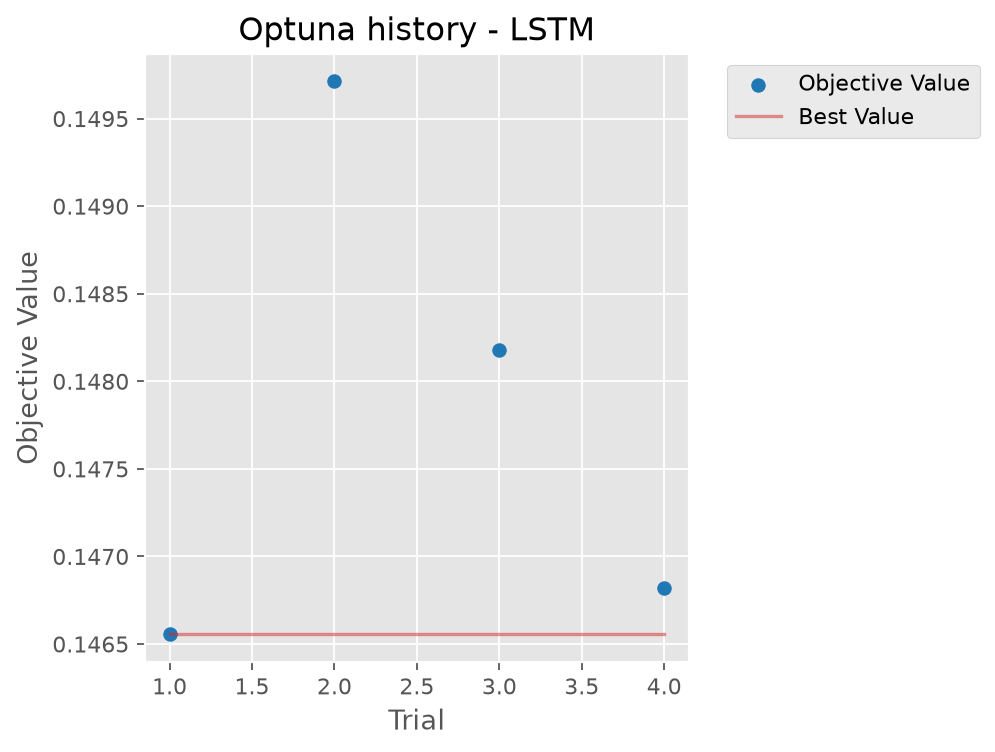
\includegraphics[width=0.55\textwidth]{figures/optuna_history.png}
\caption{Optuna history: tune log-loss of each completed trial and best value found.}
\label{fig:w2_optuna}
\end{figure}

The selected configuration is a 2-layer LSTM with 32 hidden units (15{,}457 parameters), $\eta = 2.29 \times 10^{-3}$ and $\lambda = 5.37 \times 10^{-4}$, whose best epoch was the 10th.

\paragraph{Decision threshold.} The model outputs a probability, and a threshold converts it into a churn / no-churn decision. Because churners are only 6.4\% of February, the default threshold of 0.5 classifies very few users as churners. The threshold is therefore selected on \texttt{tune} as the value in $\{0.01, 0.02, \dots, 0.99\}$ that maximises the F1-score of the churn class. The selected threshold is $0.28$, and it is frozen before the test.

\paragraph{Final model.} With the selected hyperparameters, the model is retrained on the whole February cohort (\texttt{fit} + \texttt{stop} + \texttt{tune}, 992{,}931 users) for the 10 epochs found during the search, with the scaling parameters refitted on all of February. This model predicts March once.

% ─────────────────────────────────────────────
\section{Test}
% ─────────────────────────────────────────────

\subsection{Metrics}

The final model is evaluated once on the March cohort (970{,}960 users, 8.99\% churners). We report two groups of metrics. Probability and ranking metrics do not depend on the threshold: \textbf{log-loss} and \textbf{Brier score} (mean squared error of the probability) measure the quality of the probabilities, and \textbf{ROC-AUC} and \textbf{average precision} (the area under the precision-recall curve) measure how well churners are ranked above non-churners. Decision metrics are computed at the threshold: \textbf{precision} (of the users flagged as churners, how many churned), \textbf{recall} (of the churners, how many were flagged), \textbf{F1-score} of the churn class, macro F1, balanced accuracy and the Matthews correlation coefficient (\textbf{MCC}), which accounts for all four cells of the confusion matrix and is informative under class imbalance. Accuracy is reported for completeness, but with 91\% non-churners a model that never predicts churn would already reach 0.91.

Table~\ref{tab:w2_test} reports the results at the threshold selected on \texttt{tune} (0.28) and, for reference, at 0.5.

\begin{table}[H]
\centering
\renewcommand{\arraystretch}{1.3}
\begin{tabular}{|l|c|c|}
\hline
\textbf{Metric} & \textbf{Threshold 0.28 (tune)} & \textbf{Threshold 0.5} \\ \hline
Log-loss            & \multicolumn{2}{c|}{0.2076} \\ \hline
Brier score         & \multicolumn{2}{c|}{0.0551} \\ \hline
ROC-AUC             & \multicolumn{2}{c|}{0.8507} \\ \hline
Average precision   & \multicolumn{2}{c|}{0.5801} \\ \hline
Accuracy            & 0.9319 & 0.9271 \\ \hline
Balanced accuracy   & 0.7455 & 0.6292 \\ \hline
Precision (churn)   & 0.6534 & 0.7780 \\ \hline
Recall (churn)      & 0.5181 & 0.2658 \\ \hline
Specificity         & 0.9728 & 0.9925 \\ \hline
F1 (churn)          & 0.5780 & 0.3962 \\ \hline
F1 (macro)          & 0.7705 & 0.6787 \\ \hline
MCC                 & 0.5458 & 0.4282 \\ \hline
Predicted churn rate & 7.13\% & 3.07\% \\ \hline
\end{tabular}
\caption{LSTM test metrics on the March cohort.}
\label{tab:w2_test}
\end{table}

The threshold selected in February transfers well to March: compared with 0.5, it almost doubles the recall (from 0.27 to 0.52) at a moderate loss of precision (from 0.78 to 0.65), and raises the churn F1 from 0.40 to 0.58 and the MCC from 0.43 to 0.55.

\subsection{Confusion Matrix}

Figure~\ref{fig:w2_confusion} shows the confusion matrix at the 0.28 threshold. The model identifies 45{,}247 of the 87{,}330 churners (51.8\%) and misses 42{,}083 (false negatives). It flags 23{,}998 of the 883{,}630 loyal customers as at risk (2.7\%, false positives). In other words, about two out of three users flagged by the model actually churn.

\begin{figure}[H]
\centering
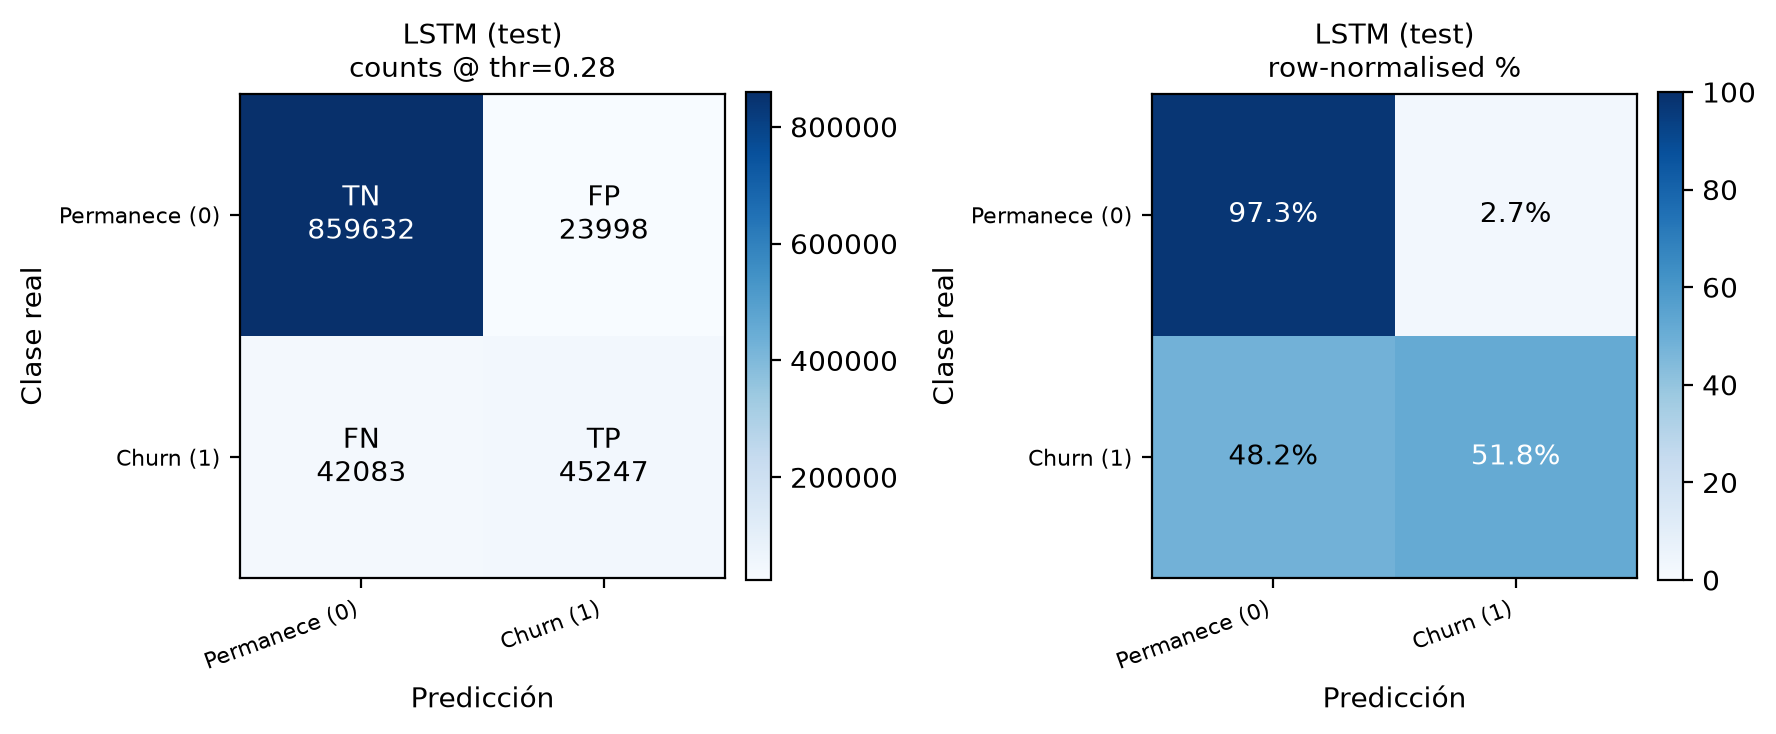
\includegraphics[width=0.9\textwidth]{figures/confusion_LSTM_test.png}
\caption{Confusion matrix on the March test cohort at the 0.28 threshold: counts (left) and percentages per true class (right).}
\label{fig:w2_confusion}
\end{figure}

\subsection{ROC and Precision-Recall Curves}

Figure~\ref{fig:w2_rocpr} shows the ROC and precision-recall curves on the test cohort. The ROC curve rises steeply at the start: the model reaches a true positive rate of about 0.7 at a false positive rate of about 0.1, so the users with the highest scores are mostly churners. The precision-recall curve keeps a precision close to 1 for the first 10\% of recall and stays above 0.6 up to a recall of about 0.55, well above the 9\% prevalence line that a random model would obtain. The drop beyond that point corresponds to churners whose 90-day behaviour looks like that of loyal customers.

\begin{figure}[H]
\centering
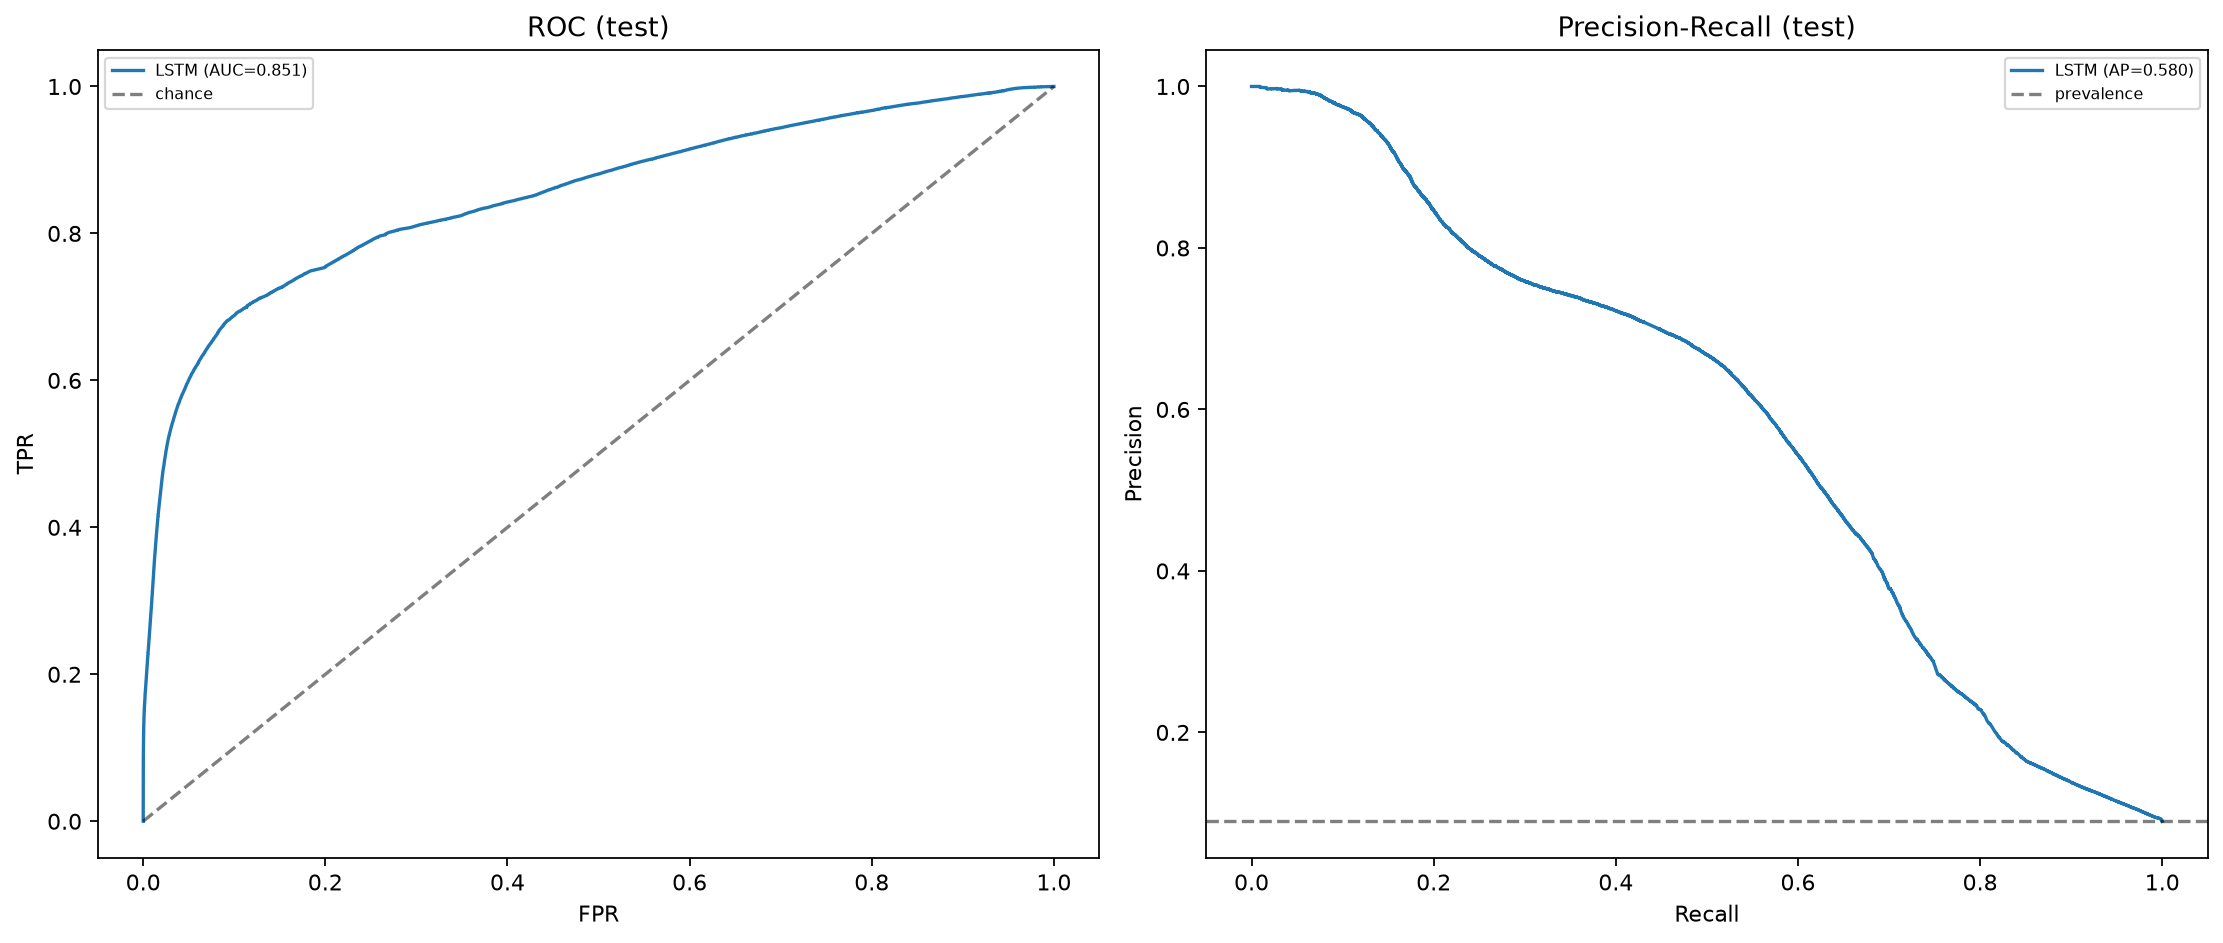
\includegraphics[width=\textwidth]{figures/roc_pr.png}
\caption{ROC curve (left, AUC = 0.851) and precision-recall curve (right, AP = 0.580) on the March test cohort.}
\label{fig:w2_rocpr}
\end{figure}

\subsection{Calibration}

Figure~\ref{fig:w2_calibration} shows the reliability diagram and the distribution of the predicted probabilities. The reliability curve lies above the diagonal: the observed churn rate is higher than the predicted probability (for example, users with a mean predicted probability of 0.45 churn at a rate of about 0.54). The model therefore underestimates churn in March. This is consistent with the change in prevalence between the two months: the model was trained on February, with 6.4\% churners, and March has 9.0\%. No calibration was applied, so this shift is reported as is.

The histogram shows that most loyal customers receive a probability close to 0, while the churners split into two groups: one spread between 0.1 and 1.0, which the model detects, and one concentrated near 0, which corresponds mostly to the false negatives of the confusion matrix.

\begin{figure}[H]
\centering
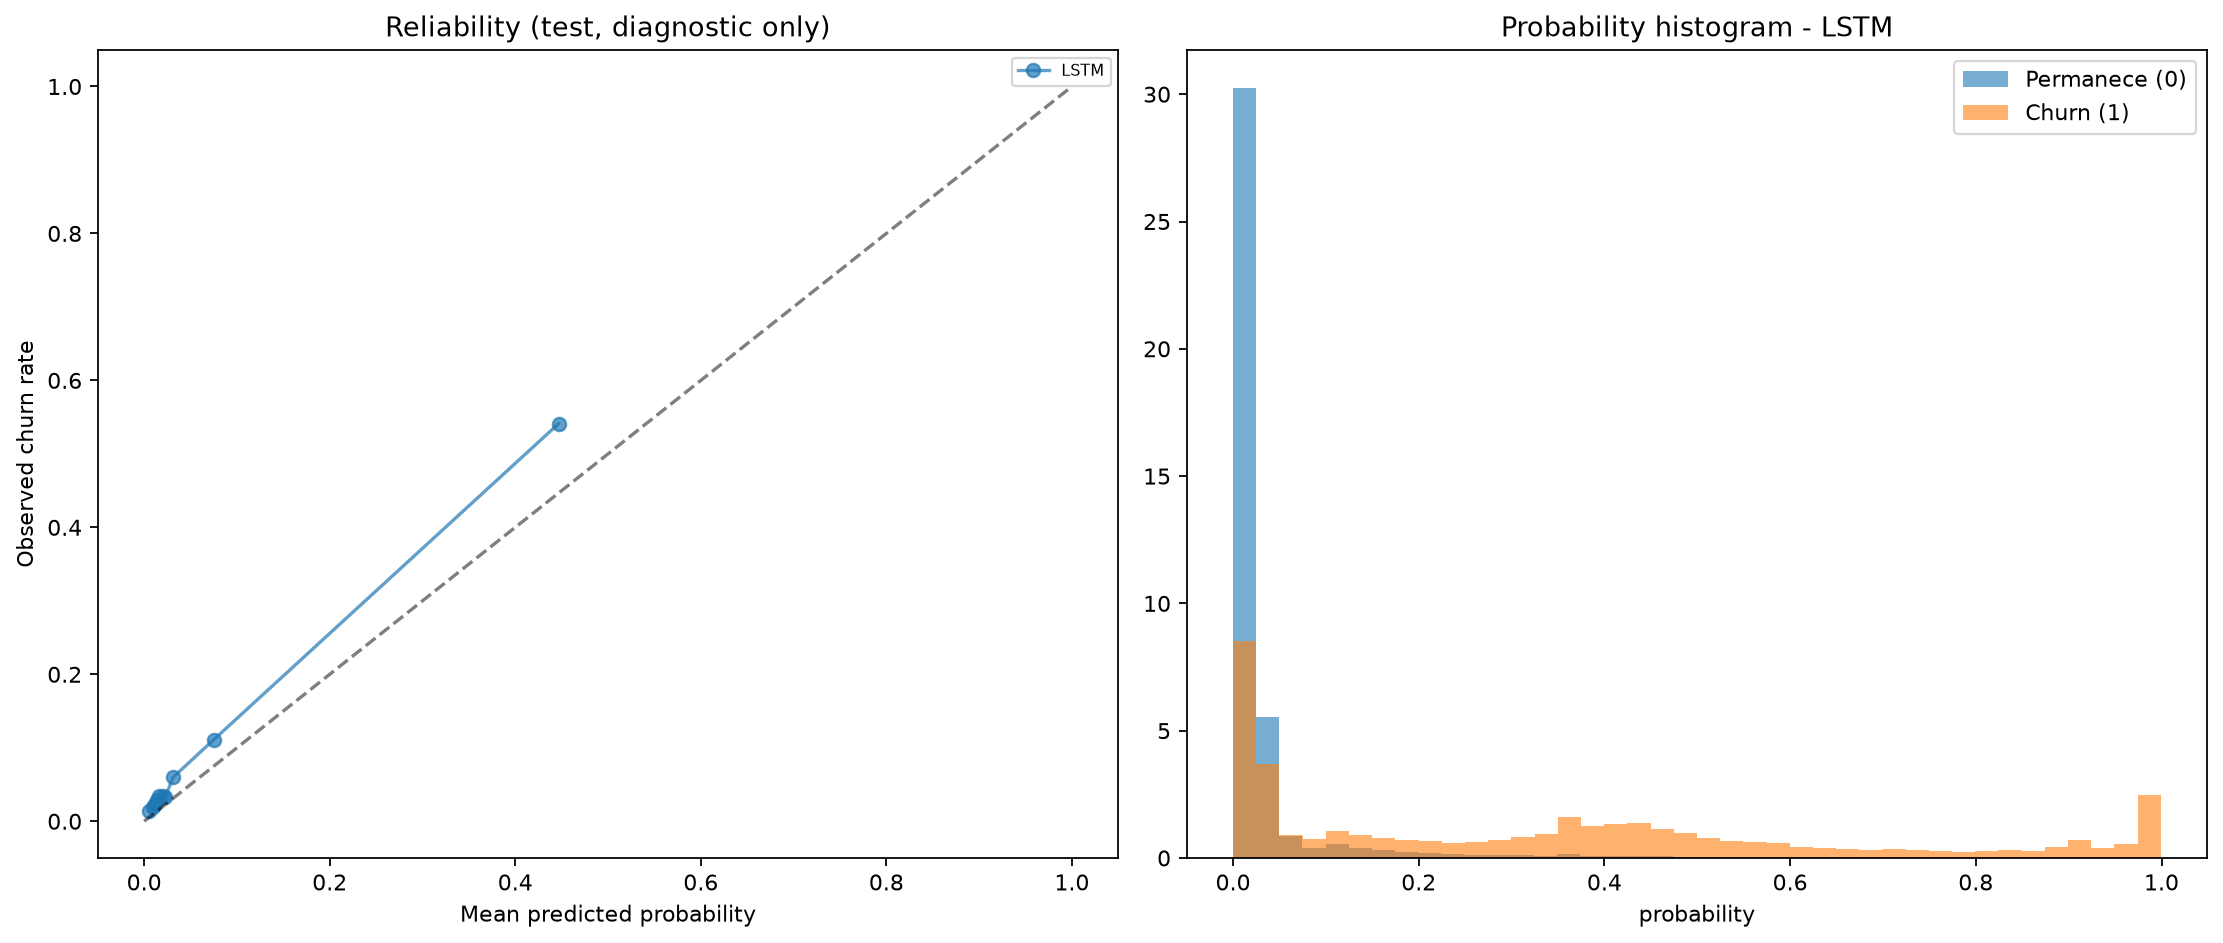
\includegraphics[width=\textwidth]{figures/calibration_hist.png}
\caption{Reliability diagram (left) and histogram of predicted probabilities by true class (right) on the March test cohort.}
\label{fig:w2_calibration}
\end{figure}

\subsection{Comparison with Workshop 1}

Table~\ref{tab:w2_vs_w1} compares the LSTM with the three tabular models of Workshop~1: logistic regression, random forest and XGBoost. All models are evaluated on the same March cohort, after selecting their thresholds on February, so the comparison is direct. The tabular models use 59 features, including member demographics and the complete transaction history; the LSTM uses only the 90-day sequences of listening and transactions, without demographics.

\begin{table}[H]
\centering
\small
\setlength{\tabcolsep}{3pt}
\renewcommand{\arraystretch}{1.3}
\begin{tabular}{|l|c|c|c|c|c|c|c|c|c|}
\hline
\textbf{Model} & \textbf{Thr.} & \textbf{Log-loss} & \textbf{Brier} & \textbf{AUC} & \textbf{AP} & \textbf{Prec.} & \textbf{Recall} & \textbf{F1} & \textbf{MCC} \\ \hline
Logistic reg. (W1) & 0.28 & 0.2126 & 0.0564 & 0.8445 & 0.5553 & 0.5811 & 0.5343 & 0.5567 & 0.5155 \\ \hline
Random forest (W1)       & 0.26 & \textbf{0.2032} & \textbf{0.0548} & \textbf{0.8632} & \textbf{0.5933} & 0.6379 & 0.5385 & \textbf{0.5840} & \textbf{0.5490} \\ \hline
XGBoost (W1)             & 0.88 & 0.4886 & 0.1498 & 0.8520 & 0.5882 & 0.6094 & \textbf{0.5424} & 0.5740 & 0.5356 \\ \hline
LSTM (W2)                & 0.28 & 0.2076 & 0.0551 & 0.8507 & 0.5801 & \textbf{0.6534} & 0.5181 & 0.5780 & 0.5458 \\ \hline
\end{tabular}
\caption{Test metrics on the March cohort for the Workshop~1 tabular models and the Workshop~2 LSTM. Each model uses the threshold selected on its own tuning partition. Best value per column in bold.}
\label{tab:w2_vs_w1}
\end{table}

The random forest remains the best model on almost every metric, but the margins are small: 0.0044 in log-loss, 0.012 in ROC-AUC, 0.006 in F1 and 0.003 in MCC. The LSTM outperforms logistic regression on every metric, and it obtains the highest precision of all models (0.653): when it flags a user as a churner, it is right more often than any tabular model, at the cost of a slightly lower recall. Against XGBoost, the LSTM is close in ROC-AUC (0.851 against 0.852) and better in F1 and MCC; it also produces much better probabilities (log-loss 0.208 against 0.489), since the XGBoost probabilities of Workshop~1 are poorly calibrated, as its 0.88 threshold reflects.

% ─────────────────────────────────────────────
\section{Conclusions}
% ─────────────────────────────────────────────

\paragraph{Relation with Workshop 1.} Workshop~1 and this workshop solve the same problem on the same data, cohorts and test month, but with two different representations. Workshop~1 summarises each subscriber into one row of 59 hand-crafted features: monthly listening aggregates, month-over-month trends, recency, transaction statistics over the complete history and member demographics. Here each subscriber is a $90 \times 20$ sequence of raw daily values, and the LSTM has to learn by itself which patterns matter. Both pipelines follow the same rules: features use only information up to each cohort cutoff, the threshold is chosen on February, and March is predicted once. This makes the results of Table~\ref{tab:w2_vs_w1} directly comparable. The LSTM reaches a performance close to the random forest (ROC-AUC 0.851 against 0.863, churn F1 0.578 against 0.584), outperforms logistic regression on every metric, and obtains the highest churn precision of all models (0.653).

\paragraph{How the sequence captures behaviour.} The LSTM reaches this performance with less information than the tabular models: only the last 90 days, without demographics and without the payment history before the window, which enters only through the state of the last pre-window payment. The daily tensor keeps the order and timing of events that the tabular features compress into monthly sums: a user who stops listening during the last two weeks, a cancellation followed by inactivity, or a membership that approaches its expiry date without a renewal. The state channels make the subscription status visible on every day, and \texttt{tx\_days\_to\_expire} turns negative when a membership expires without a new payment, which is one of the clearest churn signals. That the model reaches this performance from the raw daily sequence, without feature engineering, is the main result of this workshop; we did not analyse which of these patterns it relies on most, which would require an interpretability study. At the same time, the gap with the random forest suggests that the long-term information outside the window (tenure, full payment history and demographics) still carries predictive value that the 90-day sequence does not contain.

\paragraph{Why no further experiments are possible.} The main limitation is the dataset itself. The competition publishes official churn labels for only two months: February 2017 (\texttt{train.csv}) and March 2017 (\texttt{train\_v2.csv}). A user is labelled as churn when their membership expires in the target month and they do not subscribe again within the following 30 days, so labelling a month requires the transactions of the next 30 days. Since the published transactions and logs end on 2017-03-31, no later month (April 2017 onwards) can be labelled. Earlier months, such as January 2017 or December 2016, could in principle be labelled by applying the official labelling rule to the transactions, and the listening history before the window is available since 2015. However, our reconstruction of that rule, a port of the official \texttt{WSDMChurnLabeller.scala}, agrees with the official labels for only 98.8\% of the February users and 97.0\% of the March users, and about 137{,}000 official users per month cannot be reconstructed from the published transactions. Labels for other months would therefore be noisier than the official ones and would not define the same cohorts, so a model trained or tested on them would not be comparable with the results reported here. For this reason the evaluation is limited to one training month and one test month, and we cannot measure how stable the model is across several months.

\end{document}
